\begin{frame}
\frametitle{Curvatura}
\framesubtitle{Curvatura contínua}

Seja uma curva regular parametrizada por $t \rightarrow (x(t), y(t))$, em que $x(t)$ e $y(t)$ são funções de classe $C^2$. Sua curvatura é dada por:
$$\kappa (t) = \frac{x'(t) y''(t) - y'(t) x''(t)}{(x'(t)^2 + y'(t)^2)^{3/2}}$$   

\end{frame}

\begin{frame}
\frametitle{Curvatura discreta}
\framesubtitle{Curvatura contínua}

No caso discreto, precisa-se calcular a derivada discreta.

\medskip

Utilização de \textbf{filtro gaussiano} para suavizar e reduzir erros.

\end{frame}

\begin{frame}
\frametitle{Curvatura discreta}
\framesubtitle{Curvatura contínua}

\begin{center}
\begin{figure}
	\centering
	\begin{subfigure}[b]{0.49\textwidth}
		\centering
		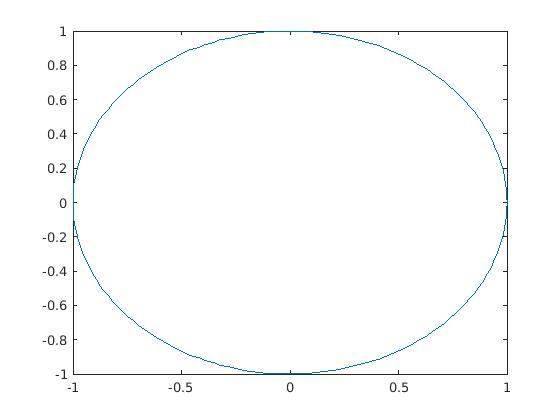
\includegraphics[width=\textwidth]{img/curva_original.jpg}
		\caption{Curva original}
		\label{fig:edic}
	\end{subfigure}
	\hfill
	\begin{subfigure}[b]{0.49\textwidth}
		\centering
		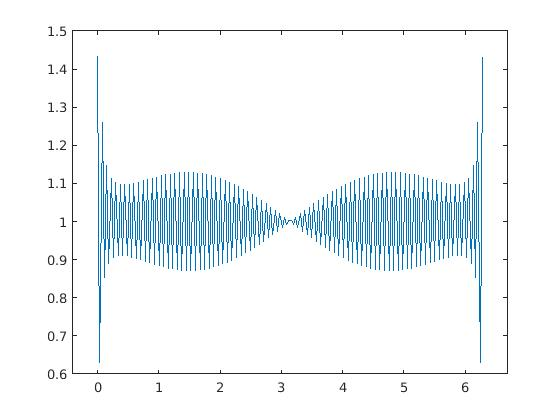
\includegraphics[width=\textwidth]{img/curvatura_calc.jpg}
		\caption{Curvatura obtida}
		\label{fig:interp}
	\end{subfigure}
\end{figure}
\end{center}

\end{frame}


\begin{frame}
	\frametitle{Curvatura discreta}
	\framesubtitle{Convolução para filtrar ruídos}
	
	\begin{center}
		\begin{figure}
			\centering
			\begin{subfigure}[b]{0.49\textwidth}
				\centering
				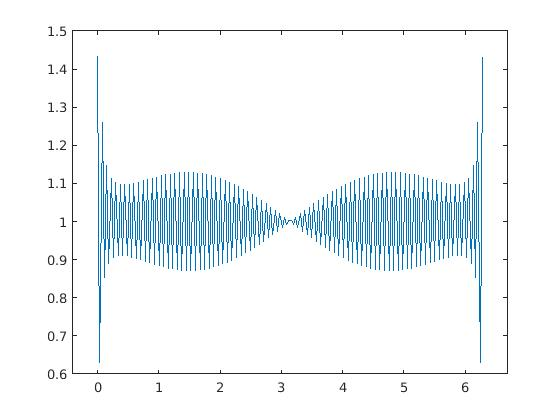
\includegraphics[width=\textwidth]{img/curvatura_calc.jpg}
				\caption{Curvatura calculada}
				\label{fig:cacurv}
				\bigskip
			\end{subfigure}
			\hfill
			\begin{subfigure}[b]{0.49\textwidth}
				\centering
				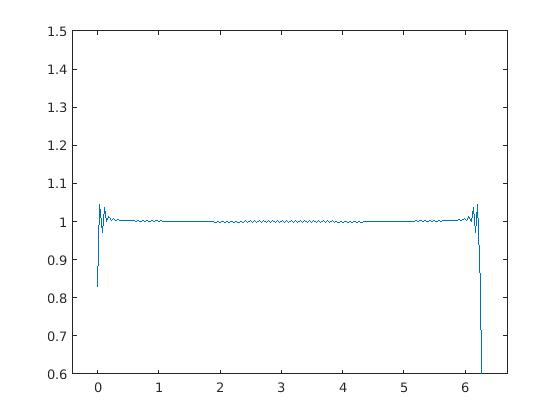
\includegraphics[width=\textwidth]{img/curvatura_arr.jpg}
				\caption{Curvatura com convolução (média dos 4 vizinhos mais próximos)}
				\label{fig:arrara}
			\end{subfigure}
		\end{figure}
	\end{center}
	
\end{frame}